\chapter{Torch implementation take-aways}\label{sec:Torch implementation}

%
%
%------- DEEP KALMAN FILTER ------------------------------
%
%

\begin{landscape}
\begin{figure}
\begin{centering}
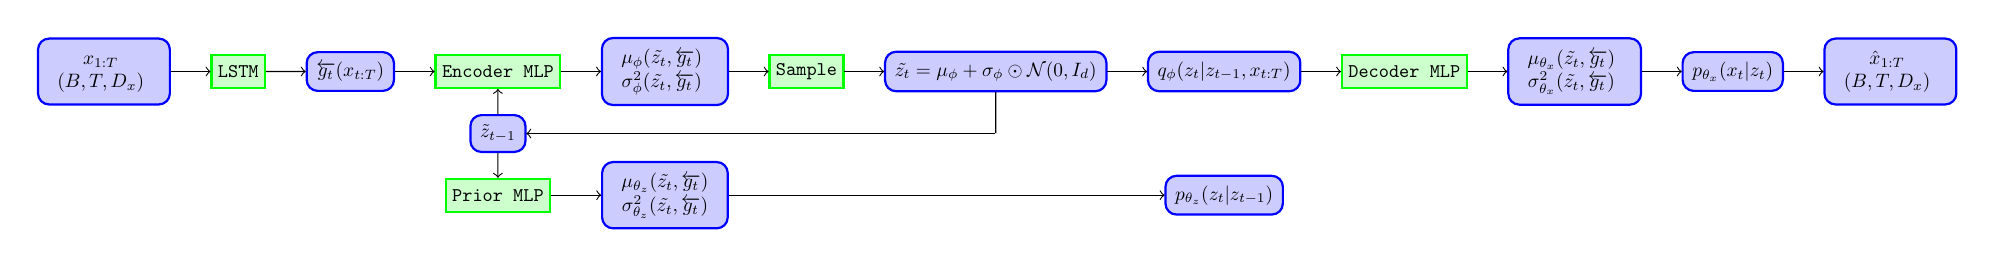
\begin{tikzpicture}[
    scale=0.70,
    every node/.style={scale=0.70},
    torch/.style={
        rectangle, 
        minimum size=6mm, 
        thick, 
        draw=green!100, 
        fill=green!20, 
        font=\ttfamily
        },
    math/.style={
        rectangle, 
        % minimum height=1cm,
        % minimum width=2cm,
        rounded corners, 
        thick, 
        draw=blue!100,
        fill=blue!20,
        align=center,
        anchor=center,
        inner sep=5pt
        },
    point/.style={
        circle,
        inner sep=0pt,
        minimum size=0pt,
        }
    ]
\matrix[row sep = 1mm, column sep=5mm] {
% first row
\node[math] (xt) {
    $\begin{array}{c}
            x_{1:T} \\
            (B,T,D_x)
    \end{array}$
}; & 
\node[torch] (lstm) {LSTM}; & 
\node[math] (gt) {$\overleftarrow{g_t}(x_{t:T})$}; &
\node[torch] (enco) {Encoder MLP}; &
\node[math] (phi) {
    $\begin{array}{c}
            \mu_{\phi}(\tilde{z_t}, \overleftarrow{g_t}) \\
            \sigma_{\phi}^2(\tilde{z_t}, \overleftarrow{g_t})
    \end{array}$
}; &
\node[torch] (sample) {Sample}; &
\node[math] (z_tilde) {$\tilde{z_t} = \mu_{\phi} + \sigma_{\phi} \odot \mathcal{N}(0, I_d)$}; &
\node[math] (q_phi) {$q_{\phi}(z_t \vert z_{t-1}, x_{t:T})$}; &
\node[torch] (deco) {Decoder MLP}; &
\node[math] (theta_x) {
    $\begin{array}{c}
        \mu_{\theta_x}(\tilde{z_t}, \overleftarrow{g_t}) \\
        \sigma_{\theta_x}^2(\tilde{z_t}, \overleftarrow{g_t})
    \end{array}$
}; &
\node[math] (p_theta_x) {$p_{\theta_x}(x_t \vert z_t)$}; &
\node[math] (x_hat) {
    $\begin{array}{c}
            \hat{x}_{1:T} \\
            (B,T,D_x)
    \end{array}$
}; \\
%second row
& & & \node[math] (z_t_1) (z_t_1) {$\tilde{z}_{t-1}$}; & & & \node[point] (coin) {}; & & &; \\
%third row
& & & \node[torch] (prior) {Prior MLP}; &
\node[math] (theta_z) {
    $\begin{array}{c}
            \mu_{\theta_z}(\tilde{z_t}, \overleftarrow{g_t}) \\
            \sigma_{\theta_z}^2(\tilde{z_t}, \overleftarrow{g_t})
    \end{array}$}; & & &
\node[math] (p_theta_z) {$p_{\theta_z}(z_t \vert z_{t-1})$}; &
& & \\
};
\path   (xt) edge [->, thin] (lstm)
        (lstm) edge [->, thin] (gt)
        (gt) edge [->, thin] (enco)
        (enco) edge [->, thin] (phi)
        (phi) edge [->, thin] (sample)
        (sample) edge [->, thin] (z_tilde)
        (z_tilde) edge [->, thin] (q_phi)
        (q_phi) edge[->, thin] (deco)
        (deco) edge [->, thin] (theta_x)
        (theta_x) edge [->, thin] (p_theta_x)
        (p_theta_x) edge [->, thin] (x_hat)
        (z_t_1) edge [->, thin] (enco)
        (prior) edge [<-, thin] (z_t_1)
        (theta_z) edge [<-, thin] (prior)
        (theta_z) edge[->, thin] (p_theta_z)
        (z_tilde) edge [-, thin] (coin)
        (coin) edge [->, thin] (z_t_1);
\end{tikzpicture}

% --- Loss DKF
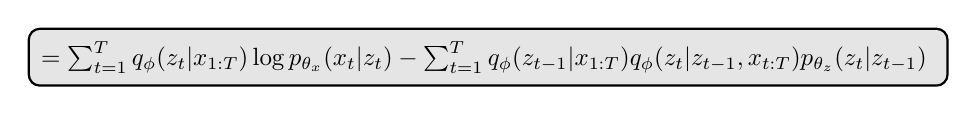
\begin{tikzpicture}[
    scale=0.90,
    every node/.style={scale=0.90},
    math/.style={
        rectangle, 
        % minimum height=1cm,
        % minimum width=2cm,
        rounded corners, 
        thick, 
        draw=black!100,
        fill=gray!20,
        align=center,
        anchor=center,
        inner sep=5pt
        },
    ]
    \node[math] {
            $\VLB = \sum_{t=1}^T \E{q_\phi(z_{t} \vert x_{1:T})} \log{p_{\theta_x}(x_t \vert z_t)} - \sum_{t=1}^T \E{q_\phi(z_{t-1} \vert x_{1:T})} \KL{q_{\phi}(z_t \vert z_{t-1}, x_{t:T})}{p_{\theta_z}(z_t \vert z_{t-1})}$
    };
\end{tikzpicture}

\end{centering}
\caption{Deep Kalman Filter Model Architecture}
\end{figure}
% \end{landscape}


%
%
% ----- VARIATIONAL RNN ------------------
%
%

% \begin{landscape}
\begin{figure}
\begin{centering}
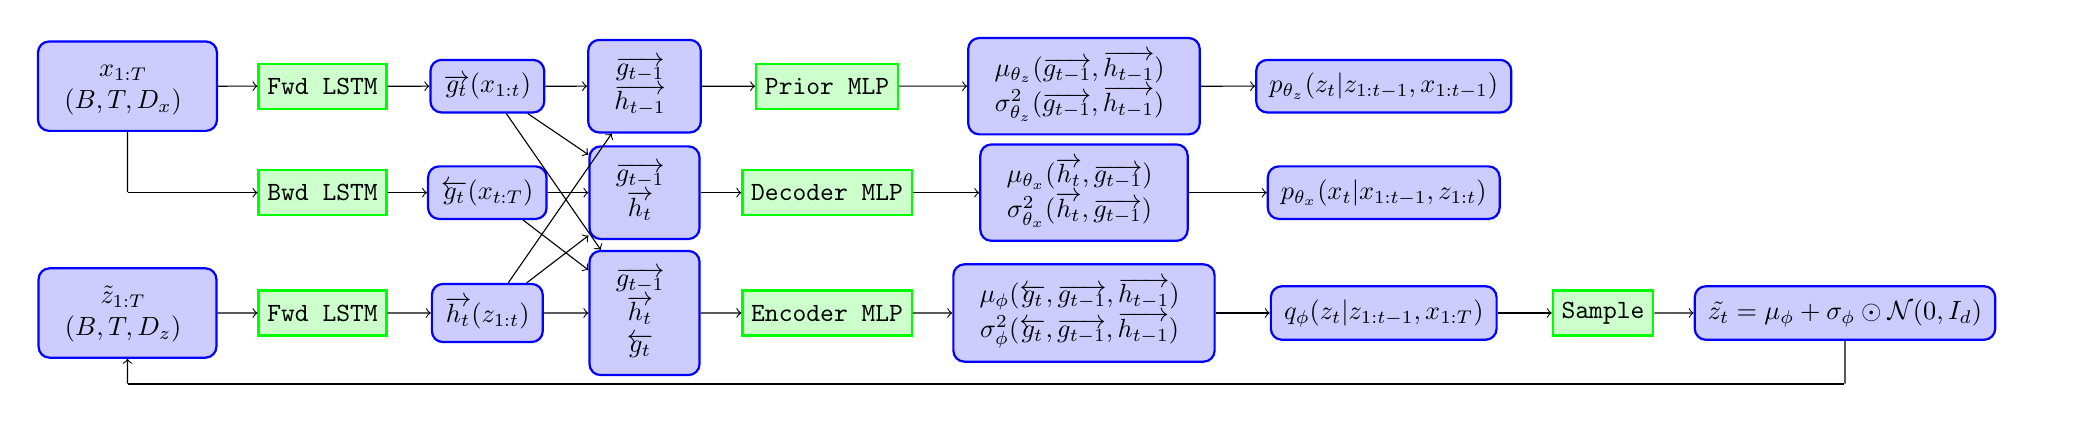
\begin{tikzpicture}[
    % format
    scale=0.95,
    every node/.style={scale=0.95},
    torch/.style={
        rectangle, 
        minimum size=6mm, 
        thick, 
        draw=green!100, 
        fill=green!20, 
        font=\ttfamily
        },
    math/.style={
        rectangle, 
        rounded corners, 
        thick, 
        draw=blue!100,
        fill=blue!20,
        align=center,
        anchor=center,
        inner sep=5pt
        },
    point/.style={
        circle,
        inner sep=0pt,
        minimum size=0pt,
        }
    ]
\matrix[row sep = 1mm, column sep=5mm] {
% row 1
\node[math] (xt) {
    $\begin{array}{c}
            x_{1:T} \\
            (B,T,D_x)
    \end{array}$
}; & 
\node[torch] (fwd_lstm) {Fwd LSTM}; & 
\node[math] (gt) {$\overrightarrow{g_t}(x_{1:t})$}; &
\node[math] (g_t_1_et_h_t_1) {
    $\begin{array}{c}
        \overrightarrow{g_{t-1}} \\
        \overrightarrow{h_{t-1}}
    \end{array}$
}; &
\node[torch] (prior) {Prior MLP}; &
\node[math] (theta_z) {
    $\begin{array}{c}
            \mu_{\theta_z}(\overrightarrow{g_{t-1}}, \overrightarrow{h_{t-1}}) \\
            \sigma_{\theta_z}^2(\overrightarrow{g_{t-1}}, \overrightarrow{h_{t-1}})
    \end{array}$
}; &
\node[math] (p_theta_z) {$p_{\theta_z}(z_t \vert z_{1:t-1}, x_{1:t-1})$}; & \\
% row 2
\node[point] (coin3) {}; &
\node[torch] (bwd_lstm) {Bwd LSTM}; & 
\node[math] (gt2) {$\overleftarrow{g_t}(x_{t:T})$}; &
\node[math] (g_t_1_et_h_t) {
    $\begin{array}{c}
        \overrightarrow{g_{t-1}} \\
        \overrightarrow{h_{t}}
    \end{array}$
}; &
\node[torch] (decoder) {Decoder MLP}; &
\node[math] (theta_x) {
    $\begin{array}{c}
            \mu_{\theta_x}(\overrightarrow{h_t}, \overrightarrow{g_{t-1}}) \\
            \sigma_{\theta_x}^2(\overrightarrow{h_t}, \overrightarrow{g_{t-1}})
    \end{array}$
}; & 
\node[math] (p_theta_x) {$p_{\theta_x}(x_t \vert x_{1:t-1}, z_{1:t} )$}; & \\
% row 3
\node[math] (z_tilde) {
    $\begin{array}{c}
            \tilde{z}_{1:T} \\
            (B,T,D_z)
    \end{array}$
}; & 
\node[torch] (fwd_lstm2) {Fwd LSTM}; & 
\node[math] (ht) {$\overrightarrow{h_t}(z_{1:t})$}; &
\node[math] (g_t_1_et_h_t_1_et_g_t) {
    $\begin{array}{c}
        \overrightarrow{g_{t-1}} \\
        \overrightarrow{h_{t}} \\
        \overleftarrow{g_t}
    \end{array}$
}; &
\node[torch] (encoder) {Encoder MLP}; &
\node[math] (phi) {
    $\begin{array}{c}
            \mu_{\phi}(\overleftarrow{g_{t}}, \overrightarrow{g_{t-1}}, \overrightarrow{h_{t-1}}) \\
            \sigma_{\phi}^2(\overleftarrow{g_{t}}, \overrightarrow{g_{t-1}}, \overrightarrow{h_{t-1}})
    \end{array}$
}; & 
\node[math] (q_phi) {$q_{\phi}(z_t \vert z_{1:t-1}, x_{1:T} )$}; &
\node[torch] (sample) {Sample}; &
\node[math] (z_tilde_formula) {$\tilde{z_t} = \mu_{\phi} + \sigma_{\phi} \odot \mathcal{N}(0, I_d)$}; & \\
% row 4
\node[point] (coin1) {};
& & & & & & & &;
\node[point] (coin2) {}; & \\
};
\path   (xt) edge [->, thin] (fwd_lstm)
        (xt) edge[-, thin] (coin3)
        (fwd_lstm) edge [->, thin] (gt)
        (gt) edge[->, thin] (g_t_1_et_h_t_1)
        (gt) edge[->, thin] (g_t_1_et_h_t)
        (gt) edge[->, thin] (g_t_1_et_h_t_1_et_g_t)
        (g_t_1_et_h_t_1) edge[->, thin] (prior)
        (prior) edge[->, thin] (theta_z)
        (theta_z) edge[->, thin] (p_theta_z)
        (coin3) edge[->, thin] (bwd_lstm)
        (bwd_lstm) edge[->, thin] (gt2)
        (gt2) edge[->, thin] (g_t_1_et_h_t)
        (gt2) edge[->, thin] (g_t_1_et_h_t_1_et_g_t)
        (g_t_1_et_h_t) edge[->, thin] (decoder)
        (decoder) edge[->, thin] (theta_x)
        (theta_x) edge[->, thin] (p_theta_x)
        (z_tilde) edge[->, thin] (fwd_lstm2)
        (fwd_lstm2) edge[->, thin] (ht)
        (ht) edge[->, thin] (g_t_1_et_h_t_1_et_g_t)
        (ht) edge[->, thin] (g_t_1_et_h_t)
        (ht) edge[->, thin] (g_t_1_et_h_t_1)
        (g_t_1_et_h_t_1_et_g_t) edge[->, thin] (encoder)
        (encoder) edge[->, thin] (phi)
        (phi) edge[->, thin] (q_phi)
        (q_phi) edge[->, thin] (sample)
        (sample) edge[->, thin] (z_tilde_formula)
        (z_tilde_formula) edge[-, thin] (coin2)
        (coin2) edge[-, thin] (coin1)
        (coin1) edge[->, thin] (z_tilde);
\end{tikzpicture}

% --- Loss VRNN
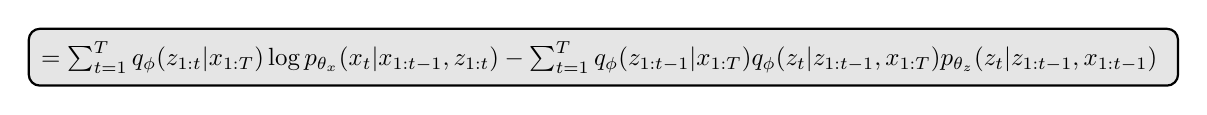
\begin{tikzpicture}[
    scale=0.90,
    every node/.style={scale=0.90},
    math/.style={
        rectangle, 
        % minimum height=1cm,
        % minimum width=2cm,
        rounded corners, 
        thick, 
        draw=black!100,
        fill=gray!20,
        align=center,
        anchor=center,
        inner sep=5pt
        },
    ]
    \node[math] {
        $\VLB = \sum_{t=1}^T  \E{q_{\phi}(z_{1:t} \vert x_{1:T})} \log{p_{\theta_x}(x_t \vert x_{1:t-1}, z_{1:t})} - \sum_{t=1}^T \E{q_{\phi}(z_{1:t-1} \vert x_{1:T})} \KL{q_{\phi}(z_t \vert z_{1:t-1}, x_{1:T})}{p_{\theta_z}(z_t \vert z_{1:t-1}, x_{1:t-1})}$
    };
\end{tikzpicture}

\end{centering}
\caption{Variational RNN Model Architecture}
\end{figure}

\end{landscape}
